To give credibility to the approach mentioned in Chapter 3, a simple test case to test the capabilities of HTM and confirm that they apply on a video is introduced.
\section{Bouncing Ball Test}

\begin{figure}[H]
    \centering
    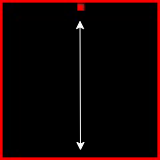
\includegraphics[width=.3\textwidth]{resources/experiments/bouncing_ball/bb_updown1.png}\hfill
    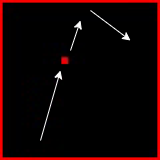
\includegraphics[width=.3\textwidth]{resources/experiments/bouncing_ball/bb_updownside.png}\hfill
    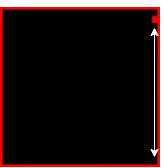
\includegraphics[width=.3\textwidth]{resources/experiments/bouncing_ball/bb_updown2.png}
    \caption{The bouncing ball test, and its three stages}
    \label{fig:bb}
\end{figure}
The video consists of a ball bouncing up and down until an anomaly occurs in the form of a sudden introduction of a horizontal velocity. After a while this horizontal velocity is set back to 0 and the ball is once again bouncing up and down in-place.
\begin{figure}[H]
    \centering
    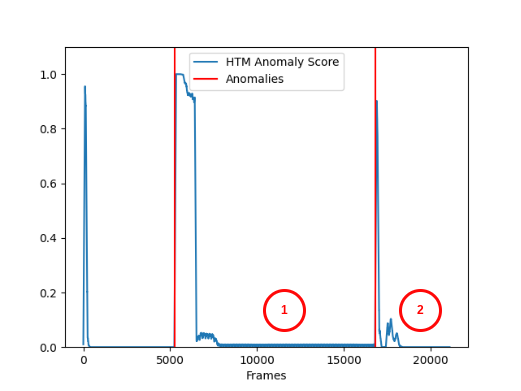
\includegraphics[width=\textwidth]{resources/experiments/bouncing_ball/bb_anoms_bad.png}
    \caption{The 100-point moving average of the anomaly score in the bouncing ball experiment.}
\end{figure}
From the figure it can be observed that it correctly detects anomalies and quickly adapts to them. On the other hand, the result is not perfect due to the minor oscillations close to mark $1$ and the anomaly spikes towards the end close to mark $2$. While the imperfections are not major and can be safely ignored, it is still important to understand their cases and what can be done to improve upon them. \par
The reason for the oscillations is due to the spatial pooler being dominated by a lucky few columns. The solution is to enable boosting. This also helped with the spikes towards the end.\par
\begin{figure}[H]
    \centering
    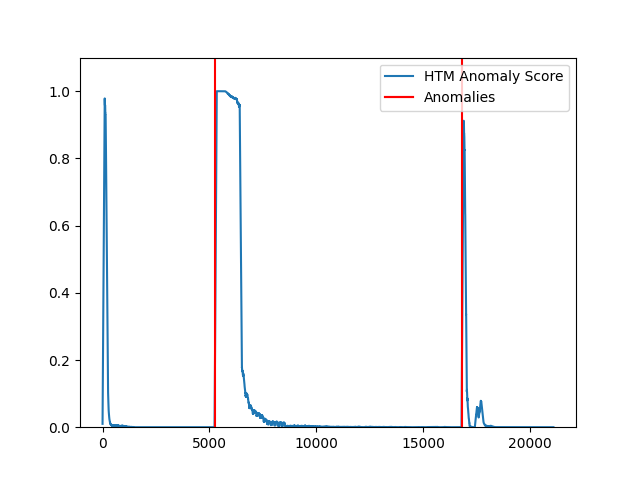
\includegraphics[width=\textwidth]{resources/experiments/bouncing_ball/bb_anoms_boosting.png}
    \caption{Bouncing ball with boosting enabled.}
\end{figure}
The reason for the anomaly spikes towards the end is because the spatial pooler had found an optimal representation when the ball was bouncing freely, but when the ball stops and starts bouncing in-place the spatial pooler ends up unlearning the old optimal representation while it learns the new optimal representation. This causes a sudden minor change in the SP output, which the TM reports as anomalous. The solution is to set the value by which permanence is decreased by to zero, effectively disabling the ability of the spatial pooler to "forget". That being said, the ability to decrement permanence is important in HTM systems, therefore disabling it is not always feasible.
\begin{figure}[H]
    \centering
    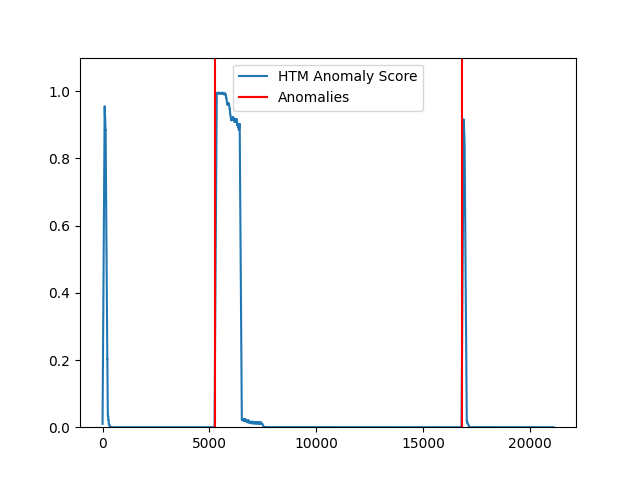
\includegraphics[width=\textwidth]{resources/experiments/bouncing_ball/bb_anoms_unforgetting.png}
    \caption{Bouncing ball without the ability of the SP to "forget".}
\end{figure}

\begin{figure}[H]
    \centering
    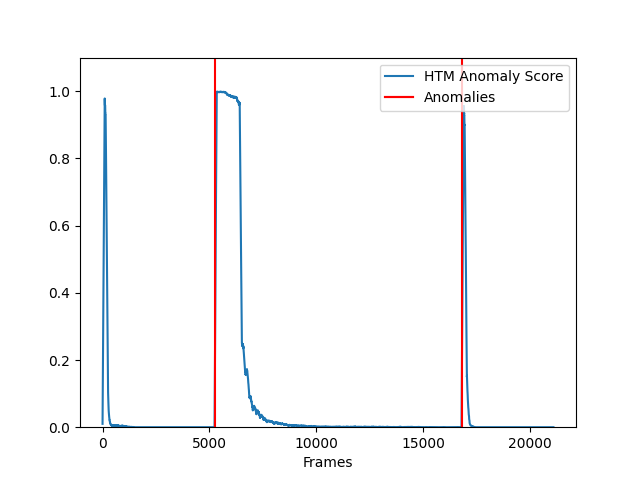
\includegraphics[width=\textwidth]{resources/experiments/bouncing_ball/bb_anoms_unforgetting_boosting.png}
    \caption{Bouncing ball without the ability of the SP to "forget" and with boosting enabled.}
\end{figure}
Final list of parameters for reproducibility:
\begin{table}[H]
    \centering
    \resizebox{\textwidth}{!}{
        \begin{tabular}{|l|l|l|}
            \hline
            \textbf{Parameter} & \textbf{Value}               & \textbf{Notes}                                      \\ \hline
            inputDimensions    & frame\_size, frame\_size     &                                                     \\ \hline
            columnDimensions   & frame\_size/2, frame\_size/2 &                                                     \\ \hline
            potentialPct       & 0.1                          &                                                     \\ \hline
            potentialRadius    & 120                          &                                                     \\ \hline
            localAreaDensity   & 0.02                         &                                                     \\ \hline
            globalInhibition   & True                         & Set to False to enable topology                     \\ \hline
            wrapAround         & True                         & \begin{tabular}[c]{@{}l@{}}Allows the columns near the \\edges to "wrap around" and form\\ connections on the other side\end{tabular}                           \\ \hline
            synPermActiveInc   & 0.1                          &                                                     \\ \hline
            synPermInactiveDec & 0                            & Set to \textgreater{}0 to enable the SP to "forget" \\ \hline
            stimulusThreshold  & 2                            &                                                     \\ \hline
            seed               & 2                            &                                                     \\ \hline
            boostStrength      & 0.1                          & Set to 0 to disable boosting                        \\ \hline
            dutyCyclePeriod    & 250                          &                                                     \\ \hline
        \end{tabular}
    }
    \caption{SP Parameters}
    \label{tab:bb_sp_params}
\end{table}
\begin{table}[H]
    \centering
    \resizebox{\textwidth}{!}{
        \begin{tabular}{|l|l|l|}
            \hline
            \textbf{Parameter}        & \textbf{Value}               & \textbf{Notes} \\ \hline
            columnDimensions          & frame\_size/2, frame\_size/2 & Same as the SP \\ \hline
            predictedSegmentDecrement & 0.003                        &                \\ \hline
            permanenceIncrement       & 0.1                          &                \\ \hline
            permanenceDecrement       & 0.001                        &                \\ \hline
            minThreshold              & 3                            &                \\ \hline
            activationThreshold       & 5                            &                \\ \hline
            cellsPerColumn            & 16                           &                \\ \hline
            seed                      & 2                            &                \\ \hline
        \end{tabular}
    }
    \caption{TM Parameters}
    \label{tab:bb_TM_params}
\end{table}
\section{Surveillance example}
\section{Sperm example}
As seen in the surveillance example, it seems the HTM can detect when segments begin and end. This experiment will explore this ability in greater detail. The dataset is INSERT HERE, which consists of videos that are made up of several segments. The sperm cells will be segmented using a rough binary thresholding.
\begin{figure}[H]
    \centering
    \begin{subfigure}[t]{0.5\textwidth}
        \centering
        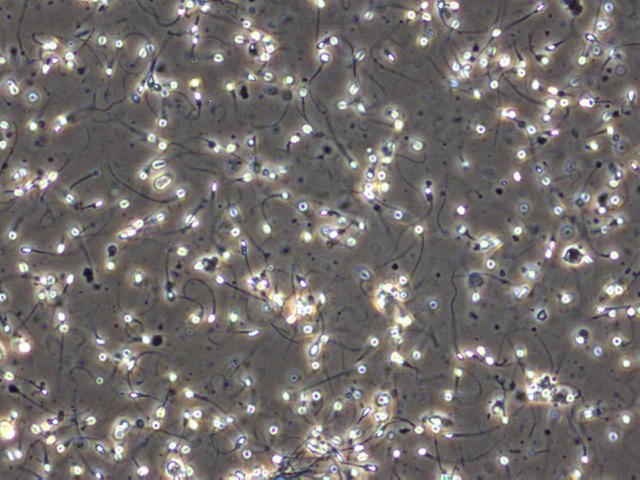
\includegraphics[width=\textwidth]{resources/experiments/sperm/sperm_example.png}
    \end{subfigure}%
    \begin{subfigure}[t]{0.5\textwidth}
        \centering
        
\includegraphics[width=\textwidth]{resources/experiments/sperm/sperm_seg_example.png}
    \end{subfigure}
    \caption{Example frame from a sperm video and its corresponding segmentation.}
\end{figure}

To ensure that the HTM does not just react to the sudden change in pixels but does something more, the L1 error will be used as a benchmark to compare against:
\begin{align*}
    E_t=\sum|F_t-F_{t-1}|
\end{align*}
Where $F_t$ denotes a segmented frame at time step $t$.
\begin{figure}[H]
    \centering
    \includegraphics[width=\textwidth]{example-image-c}
    \caption{Results.}
\end{figure}
